Poniższe wykresy przedstawiają liczbę aktywnych węzłów sieci w czasie oraz w zależności od rozmiaru pakietu i odstępie czasu pomiędzy kolejnymi pakietami. Sieć składała się z dwudziestu węzłów, które rozmieszczone zostały zgodnie z rozkładem normalnym.
Przy rozmiarach pakietu wynoszących 50B i 500B najdłuższy czas działania sieci osiągnięto wykorzystując protokół ALEACH. Czas działania sieci używających wariantów protokołu LEACH uległ wyraźnemu skróceniu przy rozmiarze pakietu wynoszącym 5000B. Wpływ okres pomiędzy pakietami na protokoły typu LEACH jest również zauważalny, jednakże jest on zdecydowanie mniej wyrazisty. Czas działania sieci dla protokołów Flood i SPIN pozostaje niezmienny, niezależnie od dobranych parametów wykresu. Dodatkowo w ich przypadku deaktywacja węzłów sieci przebiega gwałtownie oraz lawinowo - większość węzłów sieci zostaje wyłączonych w okolicach jednego punktu w czasie.

Przy rozmiarze pakietu 5B najlepszymi protokołami z punktu widzenia całkowitej długości życia sieci okazały się ALEACH oraz LEACH DCHS.

\begin{figure}[H]
	\begin{center}
		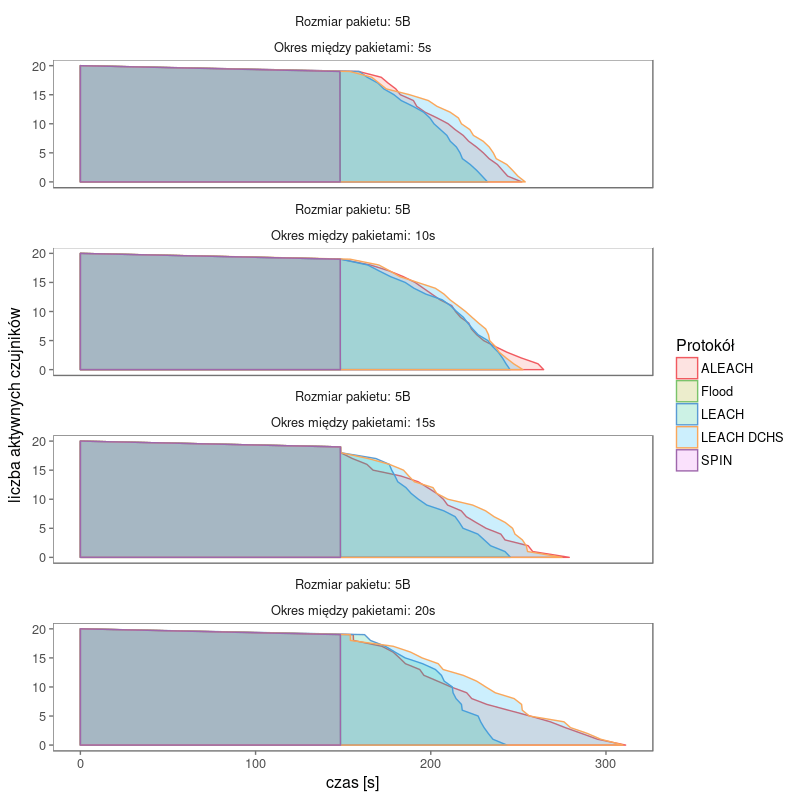
\includegraphics[scale=0.7]{\ImgPath/charts/alive_nodes_normal_20sensors_row1.png}
	\end{center}
	\caption{Aktywne węzły - 20 czujników, rozkład normalny, rozmiar pakietu: 5B}
\end{figure}

Przy rozmiarze pakietu 50B najlepszym protokołem z punktu widzenia całkowitej długości życia sieci okazał się ALEACH. W przypadku okresu między pakietami wynoszącym 20s zapewnił on około 50s dłuży czas działania sieci, jednakże protokoły LEACH oraz LEACH DCHS zapewniły dłuży okres jej stabilnego działania.

\begin{figure}[H]
	\begin{center}
		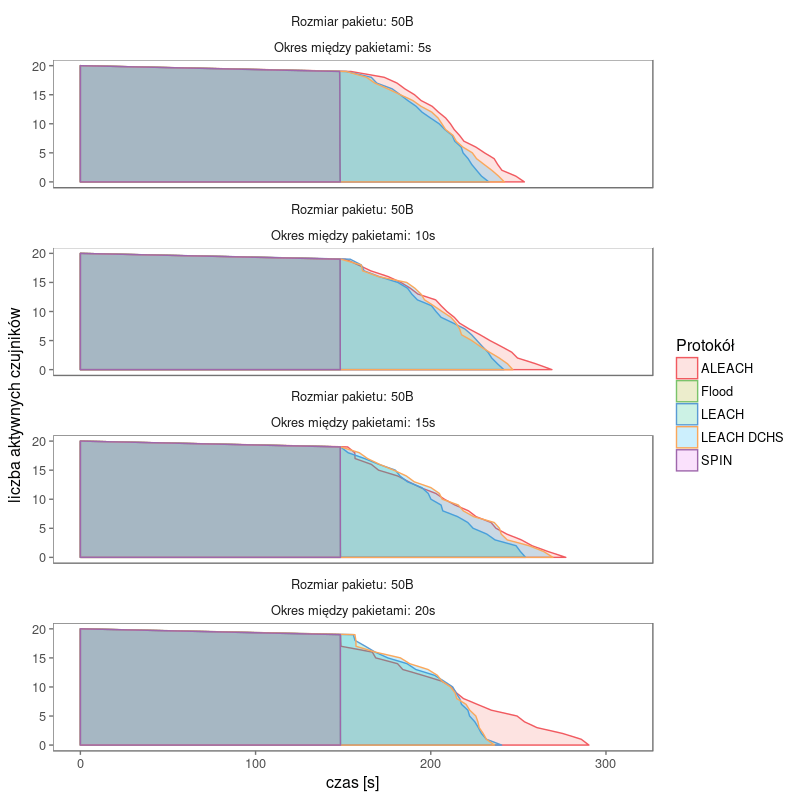
\includegraphics[scale=0.7]{\ImgPath/charts/alive_nodes_normal_20sensors_row2.png}
	\end{center}
	\caption{Aktywne węzły - 20 czujników, rozkład normalny, rozmiar pakietu: 50B}
\end{figure}

Przy rozmiarze pakietu 500B wśród protokołów umożliwiających najdłuższe działanie sieci znajduje się ALEACH. Przy okresie 10s LEACH działa lepiej od LEACH DCSH, a w przy okresie 5s i 20s LEACH DCSH działa dłużej niż LEACH.

\begin{figure}[H]
	\begin{center}
		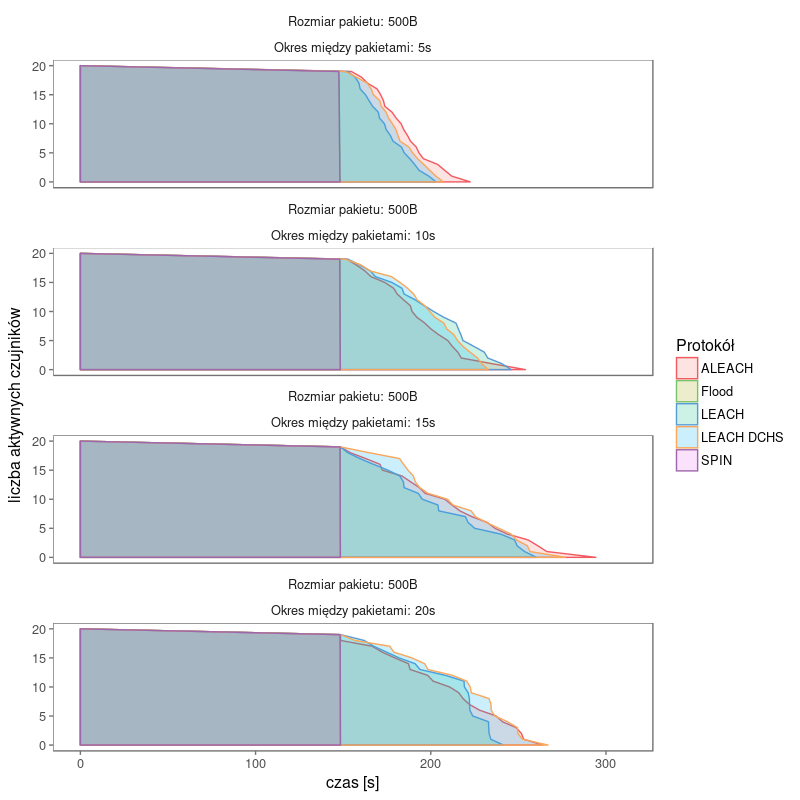
\includegraphics[scale=0.7]{\ImgPath/charts/alive_nodes_normal_20sensors_row3.png}
	\end{center}
	\caption{Aktywne węzły - 20 czujników, rozkład normalny, rozmiar pakietu: 500B}
\end{figure}

Przy rozmiarze pakietu 5000B jedynym przypadkiem w, którym ALEACH działa gorzej jest okres pomiędzy pakietami wynoszący 10s.

\begin{figure}[H]
	\begin{center}
		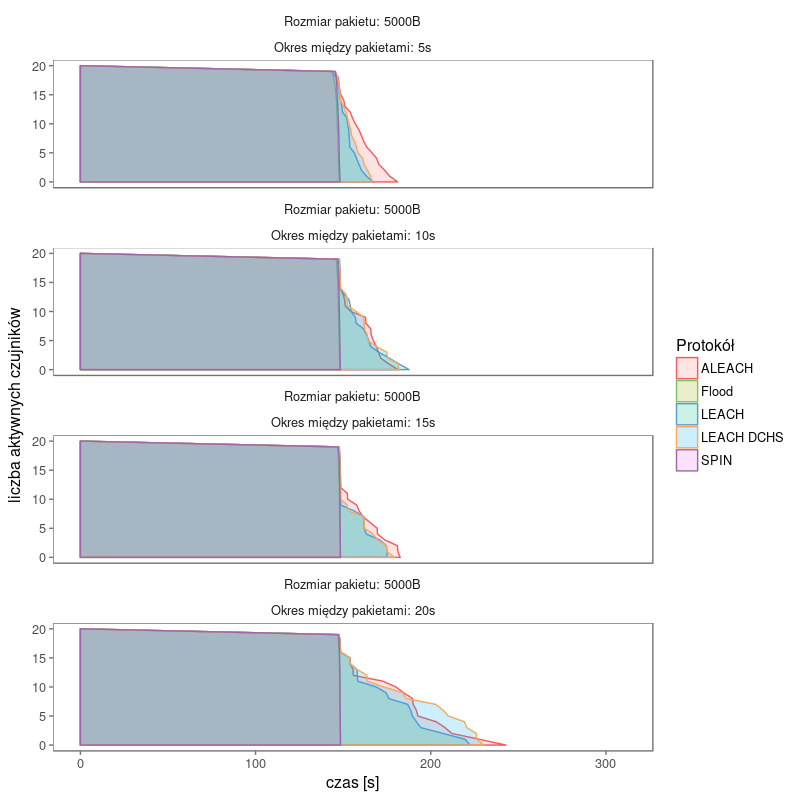
\includegraphics[scale=0.7]{\ImgPath/charts/alive_nodes_normal_20sensors_row4.png}
	\end{center}
	\caption{Aktywne węzły - 20 czujników, rozkład normalny, rozmiar pakietu: 5000B}
\end{figure}

\begin{figure}[H]
	\begin{center}
		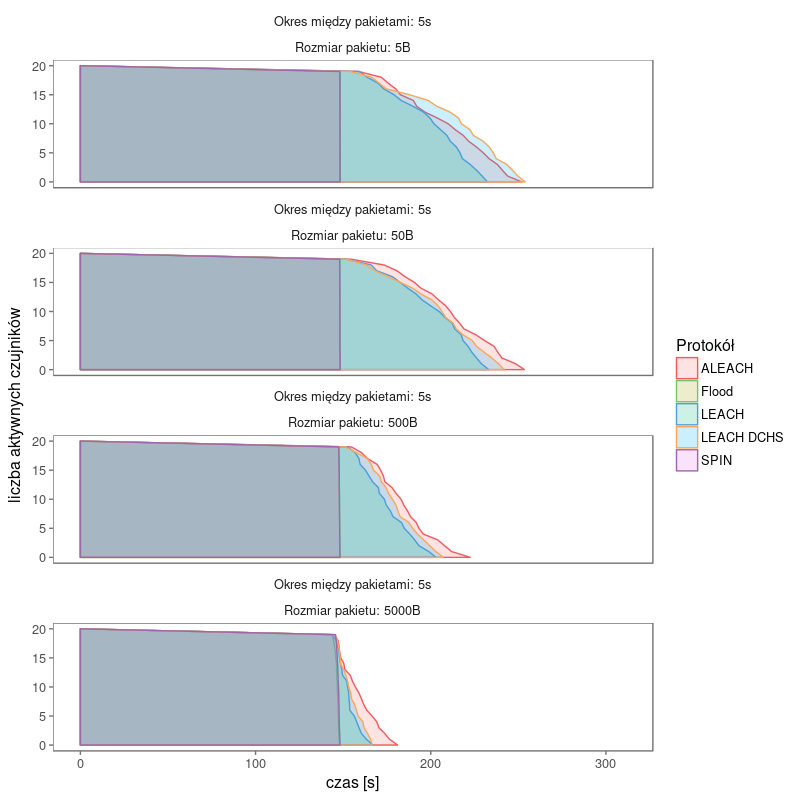
\includegraphics[scale=0.7]{\ImgPath/charts/alive_nodes_normal_20sensors_col1.png}
	\end{center}
	\caption{Aktywne węzły - 20 czujników, rozkład normalny, okres pomiędzy pakietami: 5s}
\end{figure}

\begin{figure}[H]
	\begin{center}
		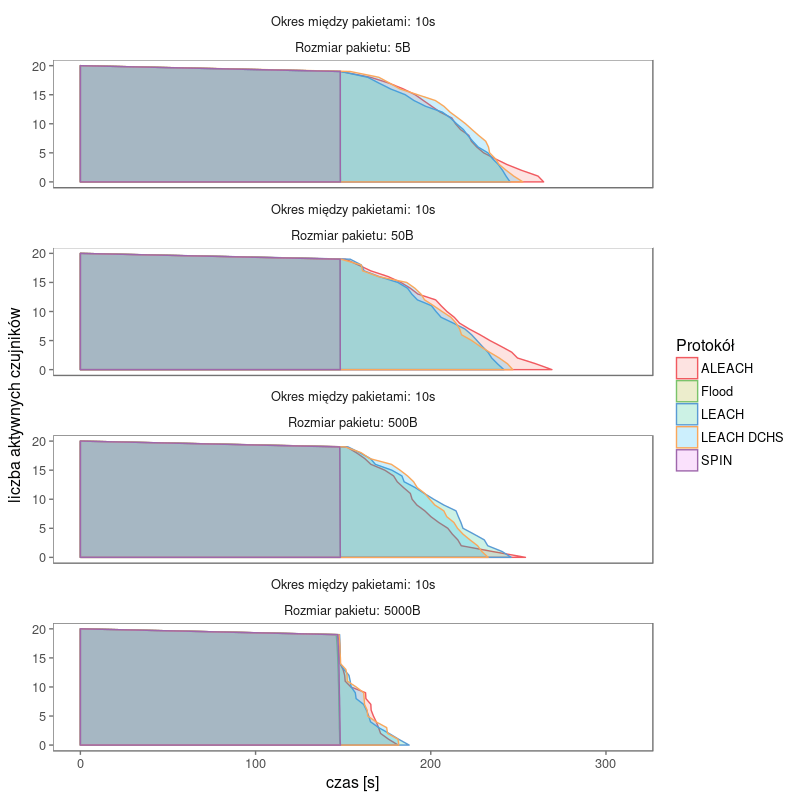
\includegraphics[scale=0.7]{\ImgPath/charts/alive_nodes_normal_20sensors_col2.png}
	\end{center}
	\caption{Aktywne węzły - 20 czujników, rozkład normalny, okres pomiędzy pakietami: 10s}
\end{figure}

\begin{figure}[H]
	\begin{center}
		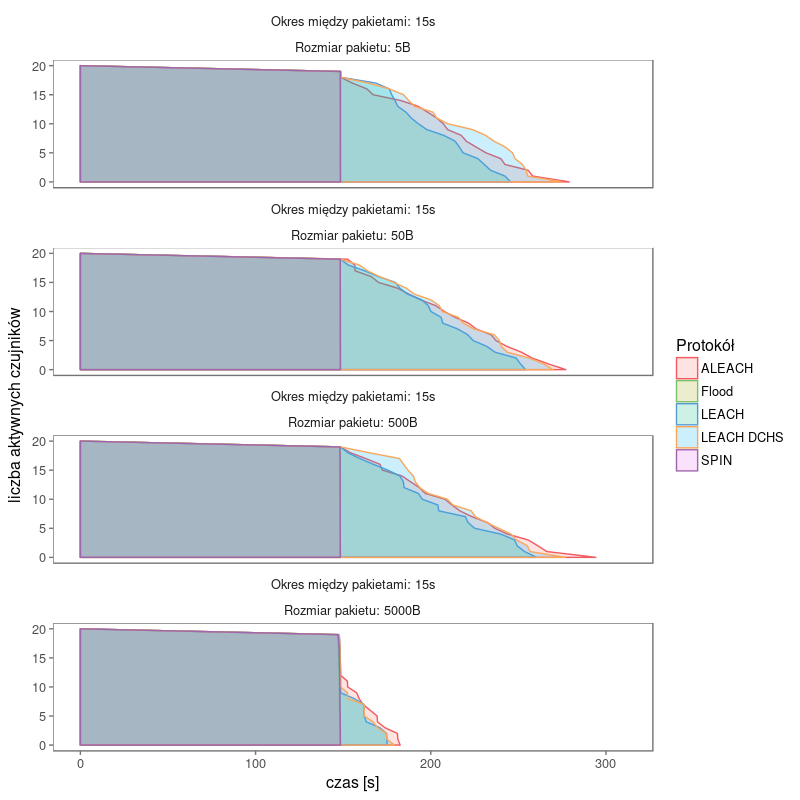
\includegraphics[scale=0.7]{\ImgPath/charts/alive_nodes_normal_20sensors_col3.png}
	\end{center}
	\caption{Aktywne węzły - 20 czujników, rozkład normalny, okres pomiędzy pakietami: 15s}
\end{figure}

\begin{figure}[H]
	\begin{center}
		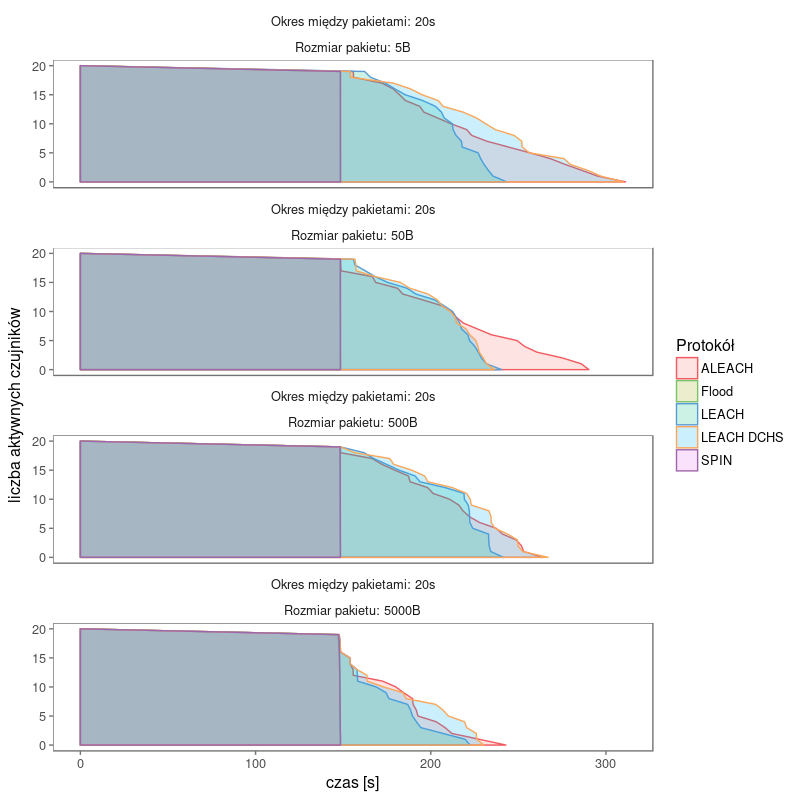
\includegraphics[scale=0.7]{\ImgPath/charts/alive_nodes_normal_20sensors_col4.png}
	\end{center}
	\caption{Aktywne węzły - 20 czujników, rozkład normalny, okres pomiędzy pakietami: 20s}
\end{figure}

\begin{figure}[H]
	\begin{center}
		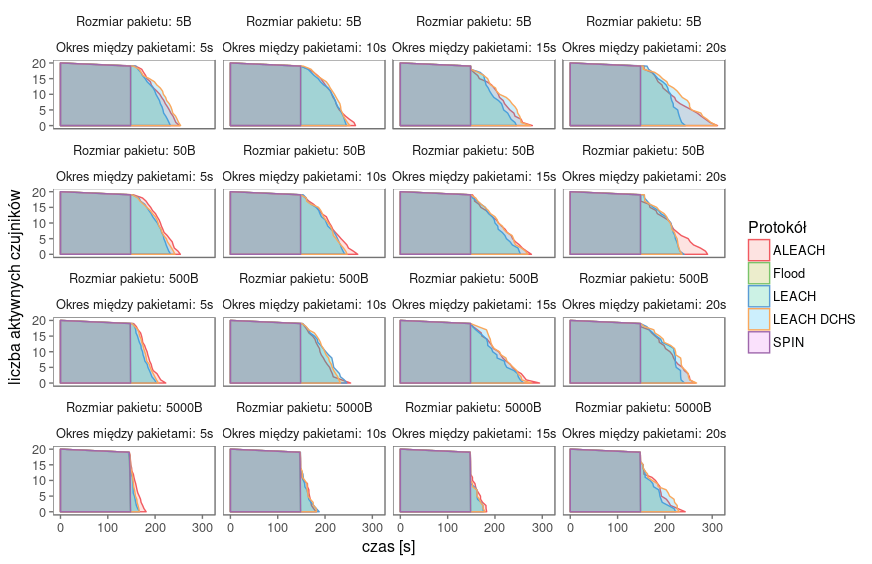
\includegraphics[scale=0.7]{\ImgPath/charts/alive_nodes_normal_20sensors.png}
	\end{center}
	\caption{Aktywne węzły - 20 czujników, rozkład normalny}
\end{figure}